\documentclass[pdflatex,compress]{beamer}

%\usetheme[dark,framenumber,totalframenumber]{ElektroITK}
\usetheme[darktitle,framenumber,totalframenumber]{ElektroITK}
\usepackage{graphicx}
\usepackage{multicol}

\title{Data Communications}

\subtitle{Introduction}

\author{Mifta Nur Farid}

\date{24 January 2024}

\begin{document}

\maketitle

\begin{frame}{Data communication}
	\begin{itemize}
		\item Data communication is the exchange of data between two devices via some form of transmission media.
		\item It depends on four characteristics:
		\begin{enumerate}
			\item Delivery:
			\item Accuracy:
			\item Timeliness:
			\item Jitter:
		\end{enumerate}
	\end{itemize}
\end{frame}

\begin{frame}{Components}
	\begin{itemize}
		\item A data communications system has five components:
		\begin{enumerate}
			\item Message
			\item Sender
			\item Receiver
			\item Transmission Medium
			\item Protocol 
		\end{enumerate}
	\end{itemize}
	\begin{center}
		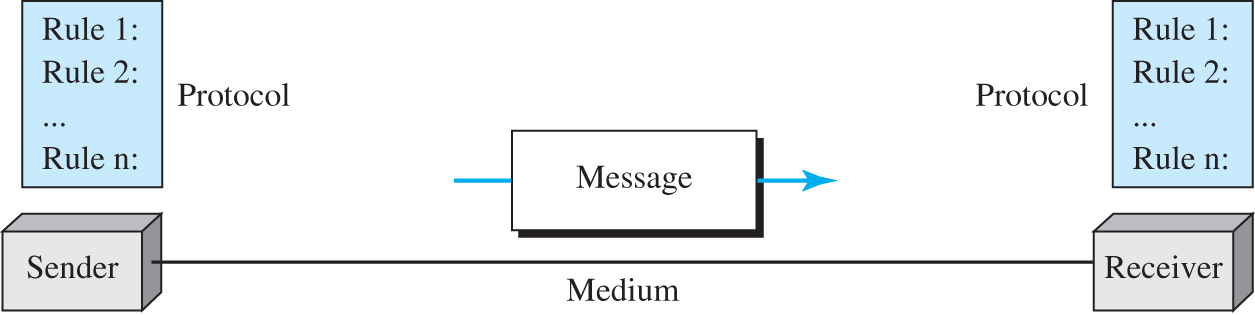
\includegraphics[width=\linewidth]{img/01}
	\end{center}
\end{frame}

\begin{frame}{Message}
	\begin{itemize}
		\item Information today comes in different forms such as text, numbers, images, audio, and video.
		\item Text is represented as a bit pattern using Unicode.
		\item Numbers are represented in binary.
		\item Images are represented as bit patterns using either RGB or YCM.
		\item Audio refers to the recording or broadcasting of sound or music, represented as analog or digital signals.
		\item Videos can be a continues images or a combination of images.
	\end{itemize}
\end{frame}

\begin{frame}{Data Flow}
	\begin{itemize}
		\item Communication between two devices can be simplex, half-duplex, and full-duplex
	\end{itemize}
	\begin{center}
		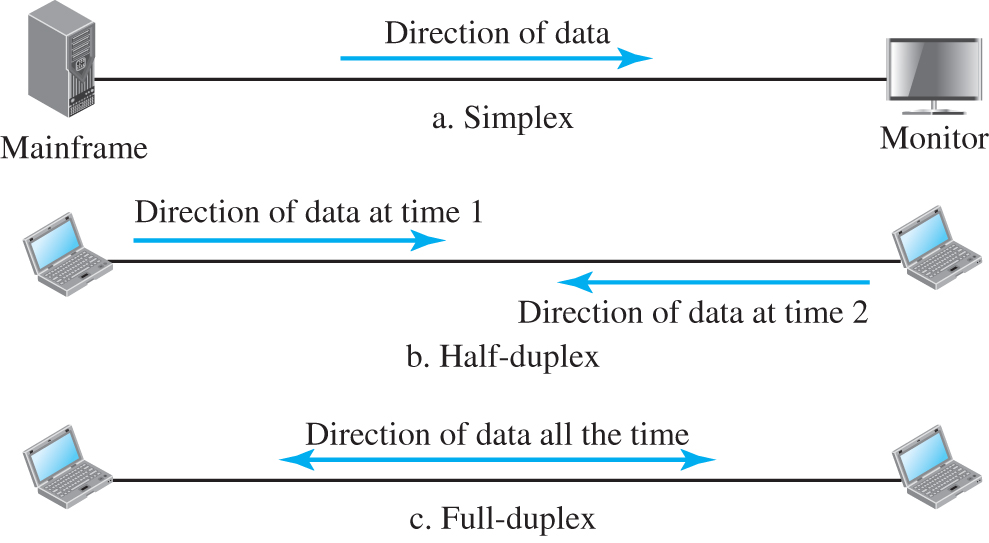
\includegraphics[width=0.9\linewidth]{img/02}
	\end{center}
\end{frame}

\begin{frame}{Network}
	\begin{itemize}
		\item A \textbf{network} is the interconnection of a set of devices capable of communication.
		\item In this definition, a device can be a \textbf{host} such as a large computer, desktop, laptop, workstation, cellular phone, or security system.
		\item A device in this definition can also be a \textbf{connecting device} such as a router a switch, a modem that changes the form of data, and so on.
	\end{itemize}
\end{frame}

\begin{frame}{Network Criteria}
	\begin{itemize}
		\item A network must be able to meet a certain number of criteria. The most important of these are: \textbf{performance}, \textbf{reliability}, and \textbf{security}.
	\end{itemize}
\end{frame}

\begin{frame}{Performance}
	\begin{itemize}
		\item Performance can be measured in many ways, including transit time and response time.
		\item Transit time is the amount of time required for a message to travel from one device to another.
		\item Response time is the elapsed time between an inquiry and a response.
	\end{itemize}
\end{frame}

\end{document}
